% Springer LNCS version (llncs class, splncs04 bibliography style). Build: latexmk -pdf main.tex
\documentclass[runningheads]{llncs}

\usepackage{amsmath,amssymb}
\usepackage{graphicx}
\usepackage{booktabs}
\usepackage{url}
\usepackage{xcolor}
\usepackage{hyperref}
\hypersetup{colorlinks=true,linkcolor=black,citecolor=black,urlcolor=blue}
\renewcommand\UrlFont{\color{blue}\rmfamily}

\setlength{\emergencystretch}{1.5em}

\begin{document}

\title{Spatial Gesture Control: Controlling a Laptop with Head Orientation and Smartwatch Pinch Gestures}
\titlerunning{Spatial Gesture Control}

\author{Vaibhav Bisht}
\authorrunning{V. Bisht}
\institute{[Department, Institution], [City, Country]\\
\email{vaibhavbisht78@gmail.com}}

\maketitle

\begin{abstract}
We present a system that lets a person control a laptop without touching it: they look at a calibrated screen location, pinch to grab a virtual volume knob, turn the wrist to change the volume and pinch again to release. Head orientation comes from consumer Sony headphones. Wrist motion and raw photoplethysmography (PPG) come from a Samsung Galaxy Watch over Bluetooth Low Energy, and all inference runs on the laptop behind a fail-closed safety chain. Because the watch cannot see the fingers, we recorded wrist signals with camera hand landmarks as reference timing annotations and evaluated detectors as continuous event detectors, counting caught pinches against false activations per hour of no-gesture time. Wrist PPG alone generalised poorly to a new day (AUC 0.60--0.64). Fusing the inertial sensors raised worst-split AUC from 0.789 to 0.837, and a three-network 1-D convolutional model on nine raw channels outperformed tree ensembles, though held-out days varied widely (43\% pooled; about two thirds on the newer days). A later model trained on hand-corrected labels caught 47 of 57 pinch-in starts with no false activations over 0.48~h on its development evaluation set, with a median latency of 442~ms. We report the system design, the data pipeline, the results and the evaluation pitfalls that inflated earlier results.

\keywords{Gesture recognition \and Smartwatch \and Photoplethysmography \and Inertial sensing \and Head tracking \and Wearable computing}
\end{abstract}

% Shared body of the paper. Included by main.tex in both the IEEE and the Springer versions.
% Wide tables use table* (two-column in IEEE, ordinary in single-column LNCS).

\section{Introduction}

Laptops are still controlled through a keyboard, a pointer or a touch surface, even though many people now wear sensors on the head and wrist all day. Noise-cancelling headphones with motion sensors know where the head points, and a smartwatch measures wrist motion and blood volume. This paper asks whether those everyday wearables can replace the keyboard for a simple spatial control: a virtual volume knob that the user looks at, grabs with a finger pinch, turns with the wrist and releases with a second pinch.

The interaction is easy to describe and hard to build. A wrist-worn watch cannot see the fingers, so a pinch must be inferred from small changes in the optical photoplethysmography (PPG) signal and in the motion sensors. Everyday movement such as typing, reaching or scratching produces similar signals, and both signals shift between days and strap fits. The three devices keep separate clocks, and the system changes a real operating-system setting, so errors must never escalate.

We built and evaluated such a system over three and a half months (27 July to 7 November 2026). Our contributions are:
\begin{itemize}
  \item A cross-platform desktop coordinator that fuses Sony headset orientation with Samsung Galaxy Watch motion and raw PPG, and drives system volume through a recipe engine with fail-closed safety.
  \item A data pipeline that records watch signals with camera hand landmarks as reference timing annotations, keeps hand corrections separate from the original labels, and trains one binary detector per gesture label.
  \item An empirical study showing that wrist PPG alone generalises poorly to new days (AUC 0.60--0.64), that adding the inertial measurement unit (IMU) raises worst-split AUC from 0.789 to 0.837, and that a small 1-D convolutional network (CNN) on nine raw channels outperforms tree ensembles on new sessions, with large day-to-day variation; a later model trained on hand-corrected labels caught 47 of 57 pinch-in starts with no false activations on its development evaluation set.
  \item An event-based evaluation standard (catches, repeats, late firings and false activations per hour of no-gesture time) applied identically in training and runtime, and a record of the evaluation pitfalls that inflated earlier results.
\end{itemize}

\section{Related Work}

\textbf{Wrist PPG gestures.} FinDroidHR classified a vocabulary including pinch from a commercial smartwatch's optical sensor~\cite{zhang2018findroidhr}, and fSense estimated gesture force from smartwatch PPG~\cite{buddhika2019fsense}. Custom hardware has recognised finger-level gestures from two green sensors~\cite{zhao2018ppg}, simple hand gestures~\cite{subramanian2020ppg} and gestures from four spatial sensor sites using principal component analysis~\cite{ruan2022pca}. Robustness studies show that sensor shift degrades PPG gesture recognition~\cite{fang2023shift} and that gesture and force level can be classified together~\cite{li2023force}. Several headline results depend on other modalities: Eddy et al.\ segment PPG gestures with accelerometer boundaries~\cite{eddy2024multimodal}, Zhao et al.'s sign-language result fuses motion sensors~\cite{zhao2021sign}, and OpenWatch reports PPG as an addition to IMU (F1 of 90\% on unseen people, with PPG adding 12.5 points)~\cite{bonazzi2026openwatch}. Multimodal wristbands~\cite{wang2022wristband,multimodal2026emg}, datasets~\cite{hauptmann2026mudpad} and force estimation~\cite{hu2026watchforce} complete the picture; reviews cover wearable gesture sensing~\cite{tchantchane2023review} and wearable PPG more broadly~\cite{charlton2023roadmap}. Most published scores evaluate prompted, pre-segmented clips, often within one user. None establishes a continuously running, low-false-activation pinch detector from stock-watch PPG.

\textbf{Motion-based pinch detection.} Tsunoda et al.\ reached 94.7\% for four gestures on unseen people using a 4{,}000~Hz accelerometer on a modified kernel, with accuracy falling sharply below 200~Hz~\cite{tsunoda2024}. ViWatch reached about 97\% over a week at 100~Hz, but 45\% on an unseen person without per-user adaptation~\cite{viwatch2023}, and Kim et al.\ detected 95\% of deliberate pinches with a threshold on the high-passed 100~Hz signal~\cite{kim2025pinch}. On the watch used here, the raw stream available to applications is 50--100~Hz for motion and 25~Hz for PPG, so the high-rate route is closed.

\textbf{Robustness methods.} We screened group distributionally robust optimisation~\cite{sagawa2019dro}, domain-adversarial training~\cite{ganin2015dann}, Deep CORAL~\cite{sun2016coral}, MiniRocket~\cite{dempster2020minirocket}, invariant risk minimisation~\cite{arjovsky2019irm} and MixStyle~\cite{zhou2021mixstyle} for cross-session robustness of PPG detectors.

\section{System Overview}

Fig.~\ref{fig:arch} shows the architecture. The headset and watch only sense; every decision runs on the laptop. The desktop application is built with Tauri~2~\cite{tauri}, a Rust backend and a React frontend. Head orientation comes from the open-source \texttt{sony-head-tracker}~\cite{sonyheadtracker}, embedded in-process on macOS and Windows and run as a UDP bridge on Linux. The Wear OS watch application streams motion and raw PPG, read through Samsung's Health Sensor SDK~\cite{samsungsdk}, to the desktop over Bluetooth Low Energy (BLE) by default, using \texttt{btleplug}~\cite{btleplug} on the desktop, or over a Wi-Fi WebSocket. A webcam running MediaPipe hand landmarks~\cite{mediapipe} is used only for labelling. Training runs offline in Python; inference runs in-process in Rust with no Python at runtime.

\begin{figure*}[t]
  \centering
  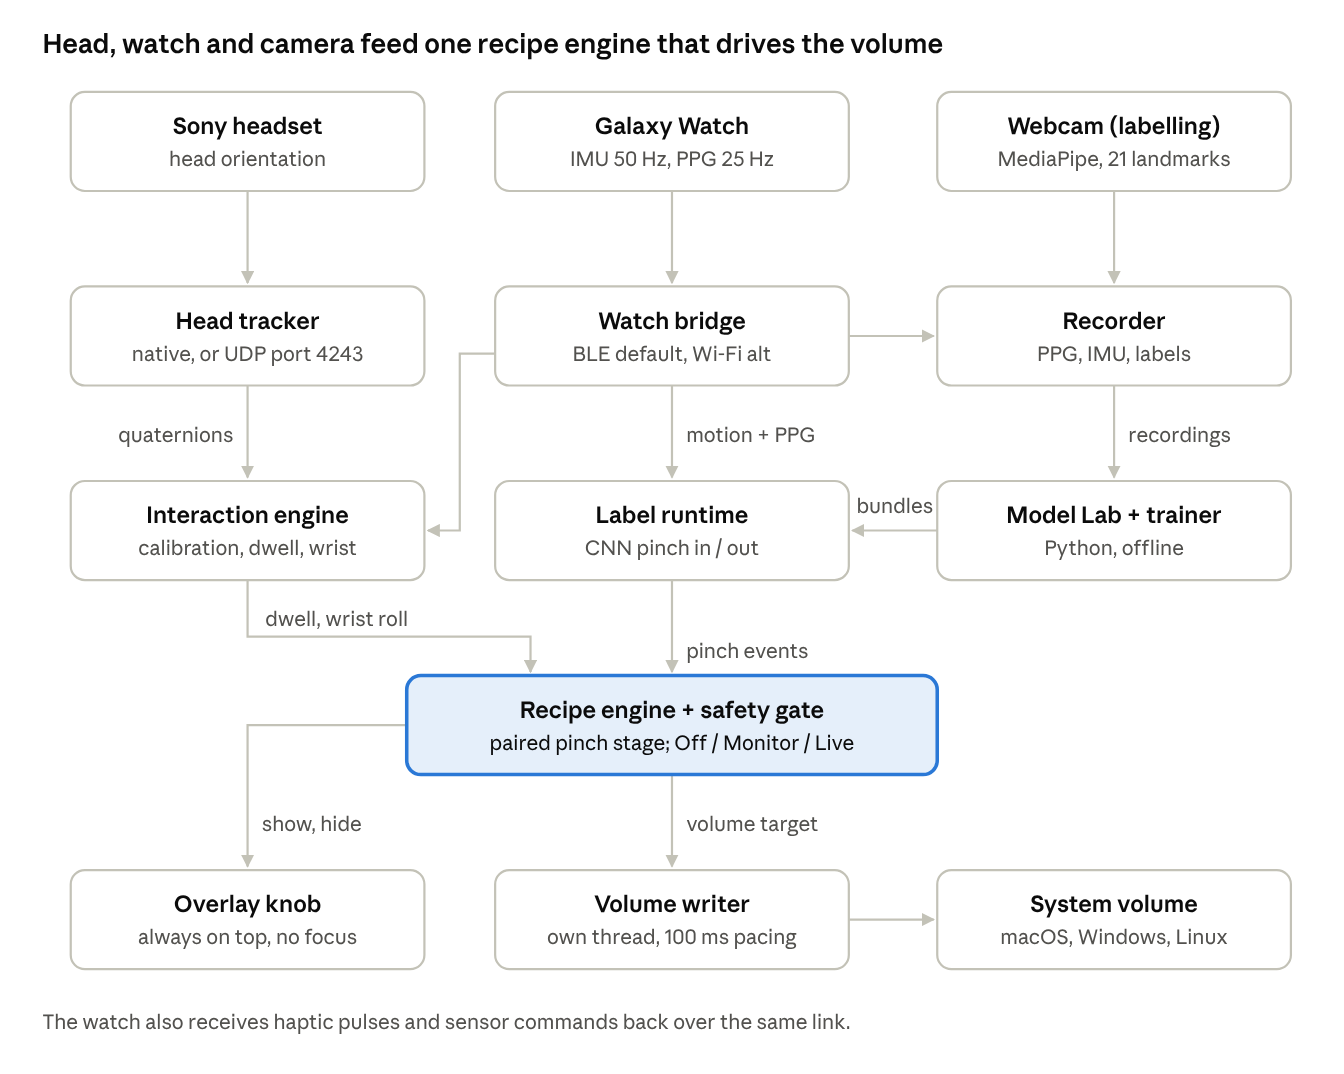
\includegraphics[width=0.82\textwidth]{architecture.png}
  \caption{System architecture. Head pose, wrist pose and pinch detections meet in one recipe engine, which alone may show the knob and drive the volume. The camera and trainer sit beside the live path.}
  \label{fig:arch}
\end{figure*}

\begin{table}[t]
  \centering
  \caption{Devices and data rates}
  \label{tab:devices}
  \small
  \begin{tabular}{@{}lll@{}}
    \toprule
    Device & Data used & Rate \\
    \midrule
    Sony headset & Orientation quaternion & $\approx$25~Hz \\
    Galaxy Watch4+ & Rot.\ vector, lin.\ accel., gyro & 50~Hz \\
                   & Raw PPG green, red, IR & 25~Hz \\
                   & Crown button, wear state & On change \\
    Webcam & 21 hand landmarks (labels only) & 23--30~fps \\
    \bottomrule
  \end{tabular}
\end{table}

The target interaction has five steps. (1) The user looks at a calibrated location (top right by default) for a dwell time of 400~ms, and a transparent, non-focusable knob appears. (2) A \emph{pinch in} grabs the knob and records the wrist pose and current volume. (3) Wrist roll changes volume relative to that pose. (4) A \emph{pinch out} releases, keeping the volume, while the knob stays ready. (5) Looking away hides the knob; Escape cancels everything.

\section{Head Targeting and Wrist Control}

\subsection{Calibration and Dwell}

The user faces the screen centre and then each named location while the system stores a unit quaternion per target. At runtime the nearest target is found by angular distance rather than separate yaw and pitch limits:
\begin{equation}
  \theta = 2\arccos\bigl(\lvert q_{\mathrm{cur}} \cdot q_{\mathrm{tgt}} \rvert\bigr),
\end{equation}
where the absolute value identifies $q$ and $-q$. A target activates when $\theta$ stays below an adjustable threshold for the dwell time. A change in the headset's reset counter means its reference frame moved, which invalidates the calibration.

\subsection{Wrist-to-Volume Mapping}

At grab time the watch orientation $Q_s$ is stored, and each new sample gives the relative rotation
\begin{equation}
  Q_{\mathrm{rel}} = Q_s^{-1} Q_{\mathrm{cur}},
\end{equation}
from which the twist about the forearm axis is extracted. The volume target is absolute from the grab pose, so errors do not accumulate. The final mapping uses a 1$^\circ$ dead zone and about one volume point per 3$^\circ$, with a sensitivity setting and a direction switch. Table~\ref{tab:filters} lists the filters. On macOS each native volume call takes 130--190~ms, so writes are applied by a dedicated thread that always takes the newest target, keeping the sensor event loop free.

\begin{table}[t]
  \centering
  \caption{Volume filters and limits}
  \label{tab:filters}
  \small
  \begin{tabular}{@{}ll@{}}
    \toprule
    Stage & Rule \\
    \midrule
    Velocity outlier & Freeze target above max.\ angular velocity \\
    Jitter rejection & Accept target changes $\geq 0.5$ points \\
    Easing & Exponential, 150~ms time constant \\
    Slew limit & $\leq 30$ points/s, independent of input rate \\
    Write pacing & $\geq 100$~ms apart, writer thread \\
    Interaction epoch & Drop writes from a released grab \\
    Clamp & 0--100 \\
    \bottomrule
  \end{tabular}
\end{table}

\section{Watch Sensing Pipeline}

The watch sends JSON envelopes (type, version, device id, sequence, timestamp, payload) over either transport, sharing one decoder. Over BLE the watch is a GATT peripheral; the desktop is the central, assigns the device identity itself and requires both OS bonding and an explicit on-watch trust approval. Motion travels in 100~ms batches and PPG at each sensor flush (default 10~Hz), about 30 BLE notifications per second in total.

Building this path exposed several faults. Fragments sized as MTU$-3 = 514$~bytes exceeded the 512-byte attribute limit, so Android silently refused every PPG batch over BLE. An unbounded queue grew to seconds of delay during arm movement, when the radio path weakens, and was then discarded whole. It was replaced by a half-second queue that drops the oldest whole messages. Sending each motion reading separately produced about 61 notifications per second, which saturated the link; batching motion and PPG as separate streams halved this. After these fixes, a 15-minute log showed 20 dropped messages (about 2~s of data), almost all just after reconnects. Timestamps stay on the watch's monotonic clock; all freshness and safety decisions use the desktop's own clock.

\section{Pinch Detection}

\subsection{Data and Reference Annotations}

Recordings are immutable bundles of PPG, IMU and labels. Pinch is split into \texttt{pinch\_in} (contact), \texttt{pinch\_hold} and \texttt{pinch\_out} (release). Fist, thumbs-up and three kinds of everyday noise (typing, mouse use and ordinary activity) are negatives. Early labels came from on-screen cues, and each recording had its own lag of up to 1.3~s. We therefore added camera reference annotations. MediaPipe~\cite{mediapipe} finds 21 hand landmarks per frame in the application's web view, without network access; only landmarks are stored. Watch timestamps and browser arrival times are logged every 200~ms, and the smallest arrival-minus-watch difference estimates the clock offset. Pinch contact is marked from finger distance. A fixed threshold of 0.35 hand sizes missed many pinches, because apparent distance depends on hand orientation; judging each session against its own hand reduced false activations on pinch sessions from 110 to 20 per hour. All recordings are from one participant's left wrist.

\subsection{Models}

Each label has its own binary model. Two kinds were developed (Table~\ref{tab:models}).

\textbf{Trees.} 2{,}733 causal features: each PPG sample is z-scored against the preceding 1, 2 and 4~s, and 21 statistics of its slope, curvature and jerk are taken over the last 0.3, 0.6 and 1.3~s (1{,}701 features). The same statistics are taken for each motion axis and its magnitude (1{,}032 features). An ExtraTrees ensemble~\cite{geurts2006extra,sklearn} of 300 trees decides about 0.88~s after a gesture starts.

\textbf{CNN.} Nine channels (accelerometer, gyroscope, PPG green, red and infrared) on a 50~Hz grid. At each decision, every channel $c$ is centred and scaled over the causal grid $G$ of the last 549 ticks (about 11~s) and the last 50 ticks $W$ (1~s) are kept:
\begin{gather}
  m_c = \operatorname{med}_{j\in G} x_{c,j}, \qquad s_c = 1.4826\,\operatorname{med}_{j\in G} \lvert x_{c,j} - m_c \rvert, \\
  u_{c,t} = \sigma\!\left(\operatorname{clip}\!\left(\frac{x_{c,t} - m_c}{s_c + \epsilon_c}, -500, 500\right)\right), \quad t \in W,
\end{gather}
where the floor $\epsilon_c$ is 0.02 for accelerometer axes, 0.01 for gyroscope axes and $0.001(\lvert m_c\rvert + 1)$ for PPG. The 450 values $u_{c,t}$ are the input. Earlier models instead z-scored each tick against the 10~s before it (Section~\ref{sec:blind}). Three dilated convolutions (32, 32 and 64 channels, kernel 5, dilation 1, 2, 4) with batch normalisation feed per-channel max and mean pooling, a 32-unit dense layer with dropout and one output. Three networks trained from different seeds are averaged. Positives are samples 0.4--0.6~s after a start; negatives are samples with no start from 1.2~s before to 0.2~s after. Training uses Adam (learning rate 0.001, weight decay 0.0001), 12 epochs and batches of 256, in PyTorch~\cite{pytorch}. The CNN decides about 0.5~s after a start.

\begin{table}[t]
  \centering
  \caption{The two detector families}
  \label{tab:models}
  \small
  \begin{tabular}{@{}lll@{}}
    \toprule
     & Trees & CNN \\
    \midrule
    Input & 2{,}733 features & $9 \times 50$ raw values \\
    Model & 300 ExtraTrees & 3 dilated 1-D CNNs \\
    Training moments & $\approx$1{,}000--1{,}300 & Tens of thousands \\
    Decision delay & $\approx$0.88~s & $\approx$0.5~s \\
    History needed & 5.6~s & 11~s \\
    \bottomrule
  \end{tabular}
\end{table}

\subsection{Detection, Thresholds and Runtime}

After the score has reached the activation threshold, a detection is emitted causally at the first strictly decreasing score (the \emph{peak} trigger); its time is that decision, not a backdated maximum. It stays active until the score falls below the release threshold, 0.15 below activation, and the 1.5~s cooldown runs from that fall. The threshold is chosen on training recordings only. Five models, each trained without one fifth of them, score the held-out parts in replay, and the threshold that catches the most starts within 30 false activations per hour is kept. Models ship as data-only bundles (tree node arrays or CNN weights) with a manifest. The SHA-256 hash and the input contract are verified on every load, and shared fixtures keep the Python and Rust input builders identical. A pinch-in detection is a one-shot event, and detector silence is not a release. A paired recipe stage therefore latches the grab on a fresh pinch-in while the head target is held, releases on pinch-out (release wins if both arrive together), and cancels on head exit, Escape, data loss, model change or leaving live mode.

\section{Evaluation Methodology}

Detectors are evaluated as continuous event detectors on whole recordings. Within each experiment, training and test recordings are disjoint, and exported files with identical sensor data are grouped as one source before splitting; one historical comparison row that reused training sessions is marked as such. Each emitted event is exactly one of: a \emph{catch} (inside the match window after a labelled start), a \emph{repeat} (another event during a caught gesture), \emph{late}, or a \emph{false activation}. The headline metrics are
\begin{gather}
  \mathrm{TAR} = \frac{\#\,\text{caught starts}}{\#\,\text{labelled starts}}, \\
  \mathrm{FAR} = \frac{\#\,\text{false activations}}{\text{hours with no gesture under way}}.
\end{gather}
The FAR denominator is deliberately not total recording time. Pinch sessions are dense, so a rate per hour of recording hid a model that fired about 175 times per hour of no-gesture time. Study designs include recording-disjoint cross-validation judged by worst-split AUC, one-shot held-out days with the protocol frozen beforehand, leave-one-day-out tests, and replays with real motion bursts spliced in. Under a constant-rate Poisson assumption, zero false activations in $T$ hours bounds the rate at about $3/T$ per hour (95\%), so short clean tests prove little.

\section{Results}

\subsection{PPG Alone Is Not Enough}

A PPG ``step'' at pinch onset appeared in every early session, but its rest controls had been chosen only by distance from gesture edges. A recheck found 84\% of them (1{,}645 of 1{,}958) inside gestures, mostly in the middle of long holds. On a one-shot held-out day (14 October 2026; 208 pinch starts and labelled non-pinch activity), every PPG onset technique scored only 0.60--0.64 AUC against non-pinch moments. None separated fist starts from pinch starts (0.37--0.57), and none was usable as a continuous detector. The PPG-only tree model fired 19--25 times per minute on recordings containing no pinch.

\subsection{Adding the IMU}

On a frozen benchmark of 37 recordings and 1{,}390 events in 20 recording-disjoint splits, fusing IMU with PPG raised worst-split AUC from 0.789 to 0.837 (better on 19 of 20 splits). It cut false activations on no-pinch recordings from 19.0 to 12.0 per minute at a threshold of 0.5. The original trigger fired at the first threshold crossing, often before the scoring window, and its lockout then blocked the correct firing. Firing at the score's peak added 4--12 recall points at the same false-activation budget, at a cost of 35--90~ms.

\subsection{CNN Against Trees}

Table~\ref{tab:lodo} reports historical leave-one-day-out results on 372 camera-marked pinches. Pooled, the selected configuration caught 161 (43\%), with strong day-to-day variation: 21/171 and 37/52 on the two October days against 67/92 and 36/57 on the two November days. On the newer sessions the CNN caught about two thirds of pinches against 10--28\% for trees, and fired about 0.4~s sooner. Applying a still-hand rule during training removed every moving moment, so the model never learned that movement is not a pinch. The best configuration trains without the rule and with everyday noise. The participant reports that pinch in and pinch out both work in the paired volume interaction.

\begin{table*}[t]
  \centering
  \caption{CNN variants, leave one day out, 372 camera-marked pinches}
  \label{tab:lodo}
  \small
  \begin{tabular}{@{}lrrr@{}}
    \toprule
    Training & Caught & FAR noise (/h) & FAR pinch (/h) \\
    \midrule
    October only, no noise (earlier)$^\ast$ & 204 (55\%) & 143 & 23 \\
    With still-hand rule & 146 (39\%) & 23 & 20 \\
    \textbf{Without the rule, with noise} & \textbf{161 (43\%)} & \textbf{7} & 49$^\dagger$ \\
    Rule only at runtime & 130 (35\%) & 3 & 16 \\
    \bottomrule
  \end{tabular}\par\smallskip
  {\footnotesize FAR noise: false activations per hour on unseen everyday-noise sessions; FAR pinch: on pinch sessions.
  $^\ast$Trained on most October pinches, so not unseen. $^\dagger$Dominated by one day; other days 0--28/h.\par}
\end{table*}

\subsection{Hand-Labelled Development Model}

Labels were later corrected by hand in the application's labelling view; a non-empty manual label overrides the original row label, and a blank one keeps it. The corrected collection has 37 exports, which reduce to 28 distinct sensor streams once identical exports are grouped. A median-scaled CNN trained on 20 of these recordings, with its 0.99 threshold chosen on training recordings only, was evaluated on eight others. Replaying the stored model (SHA-256 \texttt{ae0a22bf\ldots}) with the trainer's own detection and event-accounting code reproduced its stored metrics exactly (Table~\ref{tab:hand}). It caught 47 of 57 annotated pinch-in starts, 72--94\% by day, with four late detections, no repeats and no false activations over 0.48~h of eligible no-gesture time, and no interior input gaps. Median latency from annotated start to causal detection was 442~ms. The everyday-activity session's highest score was 0.970 against the 0.99 threshold, so the zero false-activation result rests on a narrow margin. These are development results for one participant and one target; the evaluation recordings are not established as untouched by development.

\begin{table}[t]
  \centering
  \caption{Hand-labelled pinch-in model, replay on its eight evaluation recordings}
  \label{tab:hand}
  \small
  \begin{tabular}{@{}ll@{}}
    \toprule
    Measure & Value \\
    \midrule
    Caught & 47/57 (82.5\%) \\
    Missed & 10 (4 late, 6 undetected) \\
    Repeats, false activations & 0, 0 \\
    No-gesture time & 0.48~h \\
    95\% upper bound, false act. & 6.2/h \\
    Latency, median (IQR) & 442 (384--510)~ms \\
    \bottomrule
  \end{tabular}
\end{table}

\subsection{A Normalisation Blind Spot}\label{sec:blind}

The first CNN normalised each channel by a rolling 10~s mean and standard deviation. A burst of wrist motion raised the gyroscope deviation from about 0.03 to about 1~rad/s, shrinking a following pinch about thirty-fold until the burst left the window. No training pinch had seen this: the largest 1~s gyroscope RMS before any of 459 pinch starts was 0.62~rad/s, while everyday noise reached 14~rad/s. Table~\ref{tab:hangover} summarises a window-score diagnostic: real bursts were spliced into held-out recordings and each pinch counted if the peak score 0.1--1~s after its start reached the threshold. It is not a continuous event replay or a live test, but it shows that median/MAD scaling removes the blind spot for bursts up to about 4~s.

\begin{table}[t]
  \centering
  \caption{Pinch-in window-score check after a spliced motion burst (diagnostic)}
  \label{tab:hangover}
  \small
  \begin{tabular}{@{}lrr@{}}
    \toprule
    Burst (ends 1~s before pinch) & Rolling & Median \\
    \midrule
    None & 92\% & 92\% \\
    3--6~rad/s, 2~s & 0\% & 93\% \\
    2.5--6~rad/s, 4~s & 0\% & 87\% \\
    2--6~rad/s, 6~s & 0\% & 58\% \\
    2--6~rad/s, 8~s & 0\% & 16\% \\
    \bottomrule
  \end{tabular}
\end{table}

\subsection{Other Variations}

Retraining on the model's own false alarms lowered recall (27\% against 31\%) without reducing false activations. Self-supervised pretraining raised recall at its own threshold but almost quadrupled false activations on noise (27 against 7 per hour). A 2~s input window with a fourth convolution caught 49--51\% against 45\% at about 20 false activations per hour, but its automatically chosen threshold exceeded the budget on unseen noise. A curriculum (newest clean sessions, then older camera-labelled sessions, then noise) reached 78.9\% recall for pinch-in at zero false activations on a small reserved validation pair. This is validation evidence only, not an independent test.

\section{Safety Design}

The system's external effects are bounded by a fail-closed chain. An ordering watermark, a quality gate, a window-length check, a fusion freshness check (orientation older than 500~ms is rejected) and a gesture policy each force a release when they reject data. A watchdog releases any grab whose model data has been silent for 750~ms. Inference runs in one of three modes: \emph{Off}, \emph{Monitor} (scores but never acts) or \emph{Live} (acts only through explicit intent bindings). A saved Live setting is capped to Monitor at start-up. Grabs have one owner; the web view cannot show the overlay or inject gestures; the overlay lock is never held across a native call; and model bundles are re-verified on every load.

\section{Lessons Learned}

The largest errors came from evaluation rather than code. Rest controls that were really mid-gesture, explored recordings reused as tests, and false-activation rates over the wrong denominator each made detectors look better than they were. Reference annotations mattered more than model choice: camera-timed, per-session labels removed more false activations than any architectural change. Training-time filters change what a model learns. Normalisation that looks harmless on clean data creates blind spots after realistic disturbances. On the engineering side, silently dropped BLE notifications, unbounded queues and blocking native calls each caused visible lag, and each was found by measuring before changing.

\section{Limitations and Future Work}

All data come from one participant's left wrist, mostly at 50~Hz motion, and pinches made while moving are rare in the data. Sessions recorded on 14 October remain poorly detected (12--18\%) by every model trained on other days. The best results are cross-validation and validation evidence; an untouched, multi-day test with refitted straps and long everyday negatives is still needed before any everyday false-activation claim. Physical validation on Windows and Linux, signed packaging, Wi-Fi authentication and a BLE battery trial remain open. Promising directions are per-user adaptation, which raised ViWatch from 45\% to 97\%~\cite{viwatch2023}, a longer input window with stricter threshold selection, and extending the same look-pinch-turn interaction to brightness and scrolling.

\section{Conclusion}

A headset and a smartwatch can control a laptop through a look-pinch-turn interaction. Head orientation selects the control, a CNN on watch motion and PPG detects pinch in and pinch out, and wrist roll sets the value, all behind a fail-closed safety chain. Wrist PPG alone was not sufficient on a stock watch. Motion fusion, camera-timed labels and event-based evaluation were what made the detector work.


\bibliographystyle{splncs04}
\bibliography{refs}

\end{document}
